% !TEX root = ../main.tex

\chapter{Patanalysis}
\label{ch:analysis}

\startcontents[chapters]

\vfill

\begin{alltt}\sffamily
Aidés par les moyens d'investigation de la science,
toutes les audaces d'investigation ou de conjecture,
built in simple Protestant style,
all such reasoning and from such data must.

And I style him friend,
its whole style differed materially from that of Legrand,
the calculus of Probabilities,
n'échappaient à leur investigation.

Another line of reasoning partially decided me,
to make an anatomical dissection of its body and,
ce style en débâcle et innavigable.

In a style Of gold,
que la sobriété du style se conduit de la sorte,
still a point worthy very serious investigation.
\end{alltt}

\newpage
\minicontents
\spirals

\todo{go over previous chapters incl lit review and refer back to things. bring things together. show the breadth and depth of my research!!!}
\todo{relate all of these things back to my topic of AMC}
\todo{discuss fig 6.2 (in relation to DH methodologies)}
\todo{expand 6.1 (abusing stuff, creating own rules, oulipo)}

\spirals

A lot of the more theoretical aspects of this research have been discussed in chapters~\ref{ch:foundations}\marginnote{§~\ref{ch:foundations}~\&~\ref{ch:interpretation}} and \ref{ch:interpretation}. The evaluation here is more concerned with the practical artefact \url{pata.physics.wtf} and its interpretation.

The chapter is divided into several sections addressing issues related to \url{pata.physics.wtf}. This includes a discussion of the inspirations, an analysis of some of the technical aspects, a review of design decisions made, a contextualisation and also a meta-analysis of the project's execution and management.


\section{Influences}

Looking back over the inspirations for this project described in chapter~\ref{ch:inspirations}\marginnote{§~\ref{ch:inspirations}}, some of the influences can be clearly seen straight away. Others are intentionally a bit more subtle. There are various motivations for that. First, transparency conflicts with \emph{surprise}. Serendipity was one of the original aims to try and model, so being overly obvious and descriptive about what the tool is and does would be counter productive. An element of surprise also makes it more enjoyable in repeat visits. Pure randomness is meaningless. Another reasons was \emph{humour}. Pataphysics has an intrinsic kind of humour I wanted to include in the whole presentation of the artefact. 

\begin{description}
  \item[Syzygy Surfer]\marginnote{§~\ref{s:surfer}} The influence of the Syzygy Surfer cannot be overstated. It forms the immediate predecessor to my research. It should not be forgotten that the authors of the Syzygy Surfer are part of my supervisory team. This is where the initial ideas for the pataphysical algorithms\marginnote{§~\ref{s:algorithms}} came from. There are important differences as well though. For example, pataphors were never implemented even though this was originally suggested. Also, the concept of patadata was never really conceptualised properly.\todo{explain why not} The idea of using ontologies and semantic web technologies such as \ac{RDF} to develop the system was abandoned early on too.
  \item[Faustroll Library]\marginnote{§~\ref{s:faustlib}} This fictional library of real books was direct inspiration for the Faustroll corpus used in the text search\marginnote{§~\ref{s:corpora}}. I tried my best to complete the library as accurately as I could but some of the texts where unsourceable. As with the original, I included some foreign language texts. Since the results (if the Faustroll corpus is chosen of course) are drawn from any of these texts, the mood and style of language is quite distinct and atmospheric.
  \item[Queneau's $10^{14}$ poems]\marginnote{§~\ref{s:queneau}} Queneau is another one of the inspirations that became a direct influence. The text search can be displayed as poetry\marginnote{§~\ref{s:poetry}} in the same style as Queneau's 100 thousand million poems only in digital form and with a larger set of lines. This means that many more possible poems can be generated by switching individual lines. The outcome is beautiful.
  \item[Chinese Encyclopedia]\marginnote{§~\ref{s:borges}} Borges story has been an inspiration right from the start. The subtle humour in it is great. The sort of semantic logic behind it was modeled through the pataphysical algorithms\marginnote{§~\ref{s:algorithms}}.
  \item[Yossarian]\marginnote{§~\ref{s:yossarian}} This has been interesting to watch but if anything was more of a counter inspiration. An example of what I do not want to do. Their so-called metaphoric search engine is hyped but it is wholly unclear of how their algorithm actually create these metaphors. It is hard to compare against this as it is so different even though we share some of the same goals or principles.
  \item[Library of Babel]\marginnote{§~\ref{s:babel}} The library of babel is a great project which has only indirectly influence my work. The pataphysical elements in it are obvious even though perhaps unconscious. The seriousness with which the library is presented, the pseudo-scientific approach, the vagueness of what's actually behind it. Is it random? Or is it indeed the most gigantic digital library of any book every written or even to be written? The sheer perceived scale of the library was part motivation for calculating the numbers of the generatable poems\marginnote{\faicon{table}~\ref{tab:faustshake}}.
  \item[Oulipo]\marginnote{§~\ref{s:oulipo}} Given that the \ac{OULIPO} is directly rooted in pataphysical priniciples\footnote{Remember that the \ac{OULIPO} was founded as a subcommittee of the ``Coll\`{e}ge de \'Pataphysique'' in the 60's.}, the influence on this project cannot be underestimated. The algorithms\marginnote{§~\ref{s:algorithms}} created could even be seen as an oulipian technique themselves.
  \item[Coder Culture]\marginnote{§~\ref{s:culture}} This group of inspirations is a bit more generic and influenced lots of little things throughout the project. The idea of hiding easter eggs on the site, the deliberate placement or use of errors, the obfuscation, the humour, the jargonisation and littered `l33t' style language, and the art and aesthetics behind it. All of that was influenced by coder culture---and most of all perhaps: this thesis.
\end{description}
\todo{remove yossarian criticism}


\section{Pataphysicalisation}

The internal transformation of a query term to the final results is essentially what I call the \emph{pataphysicalisation} process. The three pataphysical algorithms (Clinamen, Syzygy and Antinomy), or \emph{patalgorithms}, are at the center of this process. 

\begin{enumerate}
  \item User enters single query term,
  \item system transforms query term into list of pataphysicalised terms,
  \item system retrieves sentence fragments containing keywords from this list,
  \item system displays sentence fragments in various formats.
\end{enumerate}

It is quite interesting to compare the algorithms with each other. By removing the clutter (in this case the sentence surrounding the pataphysicalised keyword) we can see a few example results side by side below in table~\ref{tab:algorithmscomp}.

\begin{table}[!htbp]
  \begin{tabu}{X[1,L]X[3,L]X[3,L]X[2,L]}
  \toprule
  % \cline{2-4}
  \textbf{Query}
  &
  \textbf{Clinamen}
  &
  \textbf{Syzygy}
  &
  \textbf{Antinomy}
  \\ \midrule
  \textbf{clear}
  &
  altar, leaf, pleas, cellar
  &
  vanish, allow, bare, pronounce
  &
  opaque
  \\ \cmidrule{1-4}
  \textbf{solid}
  &
  sound, valid, solar, slide
  &
  block, form, matter, crystal, powder
  &
  liquid, hollow
  \\ \cmidrule{1-4}
  \textbf{books}
  &
  boot, bones, hooks, rocks, banks
  &
  dialogue, authority, record, fact
  &
  ---
  \\ \cmidrule{1-4}
  \textbf{troll}
  &
  grill, role, tell
  &
  wheel, roll, mouth, speak
  &
  ---
  \\ \cmidrule{1-4}
  \textbf{live}
  &
  love, lies, river, wave, size, bite
  &
  breathe, people, domicile, taste, see, be
  &
  recorded, dead
  \\ \bottomrule
  \end{tabu}
\caption[Comparison of patalgorithms]{Comparison of patalgorithms showing a selection of results for each.}
\label{tab:algorithmscomp}
\end{table}

Seeing the results in a table like\marginnote{\faicon{table}~\ref{tab:algorithmscomp}} this gives an almost immediate idea of how each algorithm works. This is not meant to be transparent and perhaps only after knowing the ins and outs of the algorithms can one recognise how each result was found. 

The clinamen results show words that contain one or two spelling errors of the original query term. It is perhaps counter-intuitive to have words such as `altar', `leaf' and `cellar' be classed as spelling errors of the word `clear' but they clearly could be. Remember that a spelling error can be classed in one of four ways: (1) deletion, (2) insertion, (3) substitution and (4) transposition. So, going from `clear' to `altar' is an instance of two times case 3 (`c' is replace by `a' and `e' is replaced by `t') and going from  `clear' to `leaf' is an example of case 1 (`c' is deleted) and case 3 (`r' is replaced by `f').

Looking at the second column (the syzygy results) shows the semantic relationship between the original query term and the results. Again, this may not be immediatly noticeable but certainly once you know how the process works you can recognise the common relations. This is especially evident for the antinomy algorithm which is based on opposites.

\spirals

However it is equally interesting to compare some full sentences. Looking at some of the poems at the beginning of each chapter shows the variety of the possible outcomes (see pages \pageref{ch:introduction}, \pageref{ch:inspirations}, \pageref{ch:methodology}, \pageref{ch:pataphysics}, \pageref{ch:creativity}, \pageref{ch:technology}, \pageref{ch:evaluation}, \pageref{ch:foundations}, \pageref{ch:interpretation}, \pageref{ch:implementation}, \pageref{ch:applications}, \pageref{ch:analysis}, \pageref{ch:aspirations}, and \pageref{ch:observations}). It also highlights the difference between the two corpora. Poems based on the Faustrol corpus have a very different sound and feel to it than ones based on the Shakespeare corpus.

\begin{figure}[!htbp]
\centering
\begin{minipage}{.45\linewidth}
  \settowidth{\versewidth}{earth was flat like the floor of an Oven}
  % \PoemTitle{Flower}
  \begin{verse}[\versewidth]\sffamily\footnotesize
    There was a period put to the Fire\\
    pink and spot\\
    earth was flat like the floor of an Oven\\
    as much ease as a mower doth the grass

    during the first period of my captivity\\
    room with a hard earthen floor\\
    not within everyone's power\\
    or your favourite flowers died

    shocks lose power\\
    the white daisy\\
    after a long period

    poppy\\
    peony\\
    stock to all People
  \end{verse}
\end{minipage}
\hspace{.02\linewidth}
\begin{minipage}{.45\linewidth}
  \settowidth{\versewidth}{led by their master to the flow'red fields}
  % \PoemTitle{Flower}
  \begin{verse}[\versewidth]\sffamily\footnotesize
    O bloody period\\
    I as your lover speak\\
    has she such power\\
    gather those flowers

    thy lover\\
    juiced flowers\\
    had I been any god of power\\
    or a lover's lute

    the river hath thrice flow'd\\
    but sad mortality o'ersways their power\\
    now here a period of tumultuous broils

    led by their master to the flow'red fields\\
    not a minister in his power\\
    where soulds do couch on flowers
  \end{verse}
\end{minipage}
\caption[Faustroll vs. Shakespeare poetry]{Comparison of Faustroll (left) versus Shakespeare (right) poetry, both for query term `flower'}
\label{fig:2poems}
\end{figure}

\todo{remember to replace some of the chapter poems with shakespeare}

Sometimes we can even get a general feel for the theme of the poem, as in we can recognize the connection, the relationship between the individual lines and what must be the original query term. Of course putting the poems into the chapters as they are---without specifically stating the keyword they were generated from or the corpus they are based on---makes them a bit more elusive.

The different language is quite obvious. This is helped by the fact that the Shakespeare corpus is of course written by the same author\footnote{Unless of course we believe the legends that Shakespeare didn't write those works by himself\ldots}. The Faustroll corpus contains text by over 20 different authors and in three different languages even.


\subsection{Numbers}
\label{s:numbers}

The above examples (table~\ref{tab:algorithmscomp} and figure~\ref{fig:2poems} give a good overview of the two main factors in the pataphysicalisation process, namely the three patalgorithms and the two corpora. Both only reflect a small selection of the variety of results produced though. It is therefore quite interesting to look at some actual numbers.

\begin{table}[!htbp]
  \centering
  \begin{tabu}{llcccc}
  \toprule
  \textbf{Query} & \textbf{Corpus} & \textbf{Results} & \textbf{Reverbs} & \textbf{Origins} & \textbf{Poems}\\
  \midrule
  \multirow{2}{*}{flower} & Faustroll   & 89   & 24 & 18 & \num{7.8e10}\\
                          & Shakespeare & 157  & 15 & 38 & \num{3.8e14}\\
  \cmidrule{1-6}
  \multirow{2}{*}{clear}  & Faustroll   & 542  & 79 & 23 & \num{1.3e22}\\
                          & Shakespeare & 1445 & 72 & 38 & \num{1.5e28}\\
  \cmidrule{1-6}
  \multirow{2}{*}{troll}  & Faustroll   & 124  & 16 & 16 & \num{4.4e12}\\
                          & Shakespeare & 327  & 14 & 38 & \num{1.1e19}\\
  \cmidrule{1-6}
  \multirow{2}{*}{fania}  & Faustroll   & 9    & 2  & 6  & \num{1}\\
                          & Shakespeare & 15   & 2  & 14 & \num{1}\\
  \bottomrule
  \end{tabu}
\caption[Faustroll vs Shakespeare in numbers]{Faustroll versus Shakespeare in numbers}
\label{tab:faustshake}
\end{table}

Table~\ref{tab:faustshake}\marginnote{\faicon{table}~\ref{tab:faustshake}} shows a comparison of the two different corpora with four example query terms.

\begin{description}
  \item[Results] A `result' in this case is one line (a sentence fragment). This column shows the total number of results found by the three algorithms combined. Individual results appear only once but the keyword in contains can appear in several of the results.
  \item[Reverbs] A `reverberation' is one of the terms in the list of keywords produced by the pataphysicalisation process. The list cannot contain duplicates but each reverberation cab appear in more than one result. Reverberations are used to find results in each corpus. This column shows the total number of reverberations created by the three algorithms.
  \item[Origins] An `origin' in this case is the original source text from which a given sentence fragment was retrieved. Each corpus has a set number of source texts. Each origin can contain several results based on several reverberations. This column shows the number of origins in the given corpus in which results where found.
  \item[Poems] This refers to the total number of Queneau style poems that can be generated using the given results\footnote{The original book by Queneau contains 10 sonnets with 14 lines each. This means the total number of poems producable by the book is $10^{14}$ or one hundred thousand million.}. This is calculated as the number of different options per line to the power of the number of lines.
\end{description}

To put this into perspective, the Faustroll corpus contains a total of 28 texts of very varied authors and different languages even. This might explain why not the queries in table~\ref{tab:faustshake}\marginnote{\faicon{table}~\ref{tab:faustshake}} have not found results in all of the texts. The query `clear' found results in 23 out of 28 for example while the query `fania' only found results in 6 texts. The Shakespeare corpus seems much more uniform. Reverberations generally seem to find results in all 38 source texts in the corpus apart from the query `fania'. This might be explained by the fact that Shakespeare wrote all of the texts himself using much of the same language and vocabulary unlike the Faustroll corpus. 

It is rather interesting to note that even though the Shakespeare corpus produces overall more results from more texts, the Faustroll corpus produces more reverberations per query. This might stem from the multi-author, multi-language nature of the corpus. The overall vocabulary\marginnote{§~\ref{s:index}} used is much larger than the Shakespeare one.

Regarding the final column showing the number of possible poems, let's look at the Shakespeare---clear row. There are \num{1445} number of results. These are spread over 14 lines, so each line has 103 options. The overall number of poems is therefore calculated as $103^{14}$ which equals \num{15125897248551112432256145169} (or \num{1.5e28} in short\marginnote{\faicon{table}~\ref{tab:faustshake}}).

\spirals

A slightly different angle to consider is a comparison of these kind of numbers between each of the algorithms. Table~\ref{tab:algonums}\marginnote{\faicon{table}~\ref{tab:algonums}} shows the numbers of results, reverberations and origins for the Clinamen, Syzygy and Antinomy algorithms using four example query terms (`clear', `shine', `disorder' and `stuck') for each of the two corpora (`Faustroll' and `Shakespeare').

% \todo{add french query term cœur}
\begin{table}[!htbp]
\centering\small
\begin{tabu}{ll|ccc|ccc|ccc|ccc}
\toprule
 & & \multicolumn{3}{c}{\textbf{Clinamen}} & \multicolumn{3}{c}{\textbf{Syzygy}} & \multicolumn{3}{c|}{\textbf{Antinomy}} & \multicolumn{3}{c}{} \\ 
\cmidrule{3-11}
\multicolumn{1}{l}{} & \textbf{Query} & \rotatebox{90}{Results} & \rotatebox{90}{Reverbs} & \rotatebox{90}{Origins} & \rotatebox{90}{Results} & \rotatebox{90}{Reverbs} & \rotatebox{90}{Origins} & \rotatebox{90}{Results} & \rotatebox{90}{Reverbs} & \rotatebox{90}{Origins} & \multicolumn{3}{c}{\textbf{Total}} \\ 
\midrule
\multicolumn{1}{l}{\multirow{4}{*}{\textbf{\rotatebox{90}{Faustroll}}}} 
& clear & 158 & 20 & 13 & 368 & 90 & 23 & 16 & 8 & 8 & \multicolumn{3}{c}{542---79---23} \\
\multicolumn{1}{l}{} 
& shine & 228 & 29 & 19 & 154 & 61 & 16 & 0 & 0 & 0 & \multicolumn{3}{c}{382---61---20} \\
\multicolumn{1}{l}{}
& disorder & 0 & 0 & 0 & 159 & 127 & 23 & 10 & 2 & 10 & \multicolumn{3}{c}{169---40---23} \\
\multicolumn{1}{l}{}
& stuck & 59 & 14 & 13 & 181 & 43 & 22 & 11 & 3 & 9 & \multicolumn{3}{c}{251---47---22} \\ 
\cmidrule{1-12}
\multicolumn{1}{l}{\multirow{4}{*}{\textbf{\rotatebox{90}{Shakespeare}}}}
& clear & 435 & 20 & 38 & 997 & 90 & 38 & 13 & 8 & 12 & \multicolumn{3}{c}{1445---72---38} \\
\multicolumn{1}{l}{}
& shine & 575 & 29 & 38 & 333 & 61 & 38 & 0 & 0 & 0 & \multicolumn{3}{c}{908---53---38} \\
\multicolumn{1}{l}{}
& disorder & 0 & 0 & 0 & 326 & 127 & 38 & 29 & 2 & 29 & \multicolumn{3}{c}{355---26---38} \\
\multicolumn{1}{l}{}
& stuck & 152 & 14 & 37 & 479 & 43 & 38 & 34 & 3 & 34 & \multicolumn{3}{c}{665---41---38} \\ 
\bottomrule
\end{tabu}
\caption[Numbers per algorithm]{Results-Reverberations-Origin numbers per algorithm}
\label{tab:algonums}
\end{table}

The first immediate observation surely must be that the Antinomy algorithm produces the fewest results, in two cases even none at all. This is caused by the fact that the Antinomy algorithm\marginnote{§~\ref{s:antinomy}} is based on semantic opposites in WordNet and some words simply do not have defined opposites. Addressing this issue was left for future work mentioned in chapter~\ref{ch:future}\marginnote{§~\ref{ch:future}}. On the other hand the Syzygy algorithm\marginnote{§~\ref{s:syzygy}}, which is also based on WordNet, produces most results on average.

The Clinamen algorithm\marginnote{§~\ref{s:clinamen}} interestingly produces a varying number of results depending on the query term. For the query `disorder' no results where found in either the Faustroll or the Shakespeare corpus. This of course is rooted in the fact that no reverberations where produced during the pataphysicalisation process. Here it is important to remember that the Clinamen algorithm makes use of a base document\footnote{This is hardcoded to be Jarry's \textit{Exploits and Opinions of Doctor Faustroll, Pataphysician}. Section~\ref{s:basetext} discusses what would happen if we changed the base document to something else.}\marginnote{§~\ref{s:basetext}}. Therefore the success of the algorithm depends on the vocabulary of this base text. In this particular example this means that there was no word in the base text of one or two spelling errors to the original query of `disorder'.

Looking at the origins column in table~\ref{tab:algonums}\marginnote{\faicon{table}~\ref{tab:algonums}} highlights how the Shakespeare corpus mostly produces results from each of its 38 texts. The Faustroll corpus varies a lot more. This may be due to the different languages and varying word counts of the files in the corpus.

\paragraph*{Faustroll}
\begin{itemize}
  \item There are three empty texts (Peladan, de Chilra, de Regnier).
  \item The total number of words is \num{1738461}. Of this, \num{1204158} words are from English texts (70\%), \num{497144} are French (28\%) and \num{37159} are in German (2\%).
  \item The shortest text contains \num{3853} words (Coleridge).
  \item The longest text contains \num{419456} words (Poe).
  \item The average amount of words per text is \num{62088}.
  \item The vocabulary of the index contains \num{78893} words. Of this \num{49040} are English terms.
\end{itemize}

\paragraph*{Shakespeare}
\begin{itemize}
  \item The total number of words is \num{883460}\footnote{According to \autocite{Efron1976} Shakespeare used \num{31534} different words in his works, about half of which he only used once (\num{14376}). They cite the total number of words used in his corpus as \num{884647}.}.
  \item The shortest text contains \num{2568} words (Lover's Complaint).
  \item The longest text contains \num{32031} words (Hamlet).
  \item The average amount of words per text is \num{23249}.
  \item The vocabulary of the index contains \num{23398} words.
\end{itemize}

It should be noted that the index\marginnote{§~\ref{s:index}} is generated based on the texts vocabulary minus stopwords. Stopwords (e.g. `and', `or', `the', etc.) are common terms that occur frequently in use. The full list of stopwords per language can be found in appendix~\ref{app:stopwords}\marginnote{§~\ref{app:stopwords}}.


\subsection{Sentences}
\label{s:sents}

The index stores entries in the following format (for more detail see chapter~\ref{s:index}\marginnote{§~\ref{s:index}}).

\begin{minted}{text}
{
  word1: {fileA: [pos1, pos2, ...], fileB: [pos1], ...},
  word2: {fileC: [pos1, pos2], fileK: [pos1, pos2, pos3, ...], ...},
  ...
}
\end{minted}

At the top level we have a list of words. Each word contains a list of files and each file stores a list of positions. After the pataphysicalisation process, any entries in the index that match the pataphysicalised query terms are looked up and then the corresponding sentences are retrieved to display as results. The code is set up to retrieve the first position only instead of each one (referred to as the \emph{first only} method from now on).

\begin{minted}{text}
{
  word1: {fileA: [pos1], fileB: [pos1], ...},
  word2: {fileC: [pos1], fileK: [pos1], ...},
  ...
}
\end{minted}

This has two implications: (1) there is some unnecessary computation at the startup of the program when then index is generated and (2) only a fraction of the possible results are retrieved.

The decision to only use one position was mainly made for performance issues. Generating the full results with each position (the \emph{return all} method) takes a lot more time than doing it for just the first occurance. This is perhaps best understood by looking at an example.

The Faustroll corpus produces \num{542} results for the query `clear' with only the first sentence. If we enable the retrieval of every matching sentence, the number of results increases to \num{8751}.

\begin{minted}{text}
cellar: {l_19: [4448, 18718, 68678, 110318, 192486, 267241, 352502, 352565]}
\end{minted}

The above pseudocode shows an entry for the word `cellar' with only the positions for the \py{l_19} file\footnote{Francois Rabelais: Gargantua and Pantagruel}. Another example of an index entry for the term `doctor' can be found on page~\pageref{c:pos}. The sentences for the above positions are shown below. Using only the first occurance (position) means the system ignores the rest.

\begin{itemize}
  \item rope wine is let down into a cellar
  \item bread and holy water of the cellar
  \item year who had a cool cellar under ground
  \item cellar
  \item that Nick in the dark cellar
  \item on the cellar door
  \item in mind of the painted cellar in the oldest city in the world
  \item and the painted cellar also
\end{itemize}

Table~\ref{tab:percent}\marginnote{\faicon{table}~\ref{tab:percent}} shows some example queries for both corpora and the number of results retrieved with the first position only used (as in the live version of \url{pata.physics.wtf}) in column 5 and on column 3 with all results retrieved. The final column shows what percentage of results are retrieved using the `first only' method. The average percentage for this is about 10\%. 

\begin{table}[!htbp]
\centering
\begin{tabu}{llccccc}
\toprule
 & & \multicolumn{2}{c}{\textbf{Return all}} & \multicolumn{2}{c}{\textbf{First only}} & \\
\cmidrule{3-4}\cmidrule{5-6}
\textbf{Query} & \textbf{Corpus} & \textit{Count} & \textit{Time} & \textit{Count} & \textit{Time} & \textbf{Percent} \\
\midrule
\multirow{2}{*}{clear} 
& Faustroll   & 8751    & 59s    & 542   & 1.83s   & 6.19\%  \\
& Shakespeare & 11304   & 69.2s  & 1445  & 3.59s   & 12.78\% \\
\cmidrule{1-7}
\multirow{2}{*}{solution} 
& Faustroll   & 693     & 11.7s  & 53    & 0.98s   & 7.65\%  \\
& Shakespeare & 547     & 8.51s  & 86    & 1.07s   & 15.72\% \\
\cmidrule{1-7}
\multirow{2}{*}{form} 
& Faustroll   & 19222   & 120s   & 1064  & 2.81s   & 5.54\%  \\
& Shakespeare & 13635   & 90s    & 2125  & 4.63s   & 15.58\% \\
\cmidrule{1-7}
\multirow{2}{*}{record}
& Faustroll   & 5199    & 38s    & 275   & 1.72s   & 5.29\%  \\
& Shakespeare & 7631    & 49.2s  & 794   & 2.09s   & 10.40\% \\ 
\bottomrule
\end{tabu}
\caption[Count and time of results]{Count, time and percentage of results retrieved}
\label{tab:percent}
\end{table}

Google recommends having a ``response time under 200ms''\footnote{\url{https://developers.google.com/speed/docs/insights/Server}}. The numbers in table~\ref{tab:percent}\marginnote{\faicon{table}~\ref{tab:percent}} clearly show that the `return all' method is unacceptable in terms of speed performance. Using the `first only' method is much closer to the recommended speed limit. Columns 4 and 6 show the time it takes for the page to load from the user query to the display of results. The times are shown in seconds. The data for column 4 was generated using a Chrome browser plugin called ``Load-timer'' by alex-vv\footnote{\url{https://github.com/avflance/chrome-load-timer}} and the data for column 6 was generated by the Chrome ``Developer Tools''.


\subsection{Index}
\label{s:analindex}

The index\marginnote{§~\ref{s:index}} is a central part of the \url{pata.physics.wtf} system. It is generated when the program/server is first started up but then cached and re-used. The initial process of going over all the text files in each corpus takes a few minutes. Of course in comparison to a full Internet crawl this is a tiny amoutn of data to be processed. 

The Faustroll corpus\marginnote{§~\ref{s:corpora}} for example contains 28 texts\footnote{This is technically not true since a few of those files are empty.}. Individually they are small plaintext files of sizes between 24KB (Coleridge) and 2MB (Poe). This is of course caused by the nature of some of these texts. Samuel Coleridge's \textit{The Rime of the Ancient Mariner} is a poem whereas the Edgar Allan Poe file contains a collection of all of his works. The total size of the Faustroll corpus is 10MB. The Shakespeare corpus is much more evenly distributed as all of his works are separated out into individual text files of an average size of around 150KB. The total size of the Shakespeare corpus is only 5.3MB.

Now, the size of the actual index data structure is interesting. Processing the Faustroll corpus alone produced an index of 12.4MB. That's larger than the actual size of the corpus. Remember, the index contains each word that occurs anywhere in the corpus together with the list of files it is found in and the specific locations within each text. This includes English words buts also French and German terms since the Faustroll corpus is multi-lingual. The combined index is therefore 35.2MB large.

Figure~\ref{fig:termdocs}\marginnote{\faicon{object-group}~\ref{fig:termdocs}} shows some example words and how often they occur in three example files of the Faustroll corpus in the form of a \ac{TDM} (see chapter~\ref{ch:technology} for more details). Implementing the Faustroll corpus index as a \ac{TDM} properly, would result in a $78893 \times 28$ matrix---the number of words (not counting duplicates) times the number of files in the corpus.

\spirals

As mentioned before\marginnote{§~\ref{s:index}}, the index is structured in a double nested dictionary style list as shown below.

\begin{minted}{text}
{
  word1: {fileA: [pos1, pos2, ...], fileB: [pos1], ...},
  word2: {fileC: [pos1, pos2], fileK: [pos1, pos2, pos3, ...], ...},
  ...
}
\end{minted}

There are other options of how to make this data structure. For example we could store a list of pataphysicalised query terms (\emph{patadata}) with each word and the full sentence fragment with each position. This would allow faster retrieval at query time but would increase the time needed for the initial startup. Additionally we could store data on rhyming patterns directly in the index with each word entry. This would of course be beneficial for the implementation of a rhyming scheme for the poetry generation. See also chapter~\ref{ch:future}\marginnote{§~\ref{ch:future}}.

\begin{minted}{text}
{
  word1: ([patadata], [rhymes], {fileA: [(pos1, sent), (pos2, sent), ...], fileB: [(pos1, sent)], ...}),
  word2: ([patadata], [rhymes], {fileC: [(pos1, sent), (pos2, sent)], fileK: [(pos1, sent), (pos2, sent), (pos3, sent), ...]), ...},
  ...
}
\end{minted}

\spirals

As a comparison to the 35 megabyte index generated by the system described in this thesis, and the search times mentioned in table~\ref{tab:percent}, Google claims to have ``well over 100,000,000 gigabytes'' of data in their index and that they've spent ``over one million computing hours to build it''. Similarly Google managed to retrieve about \num{2140000000} results for the query `clear' in 0.85 seconds.

\begin{quotation}
  The web is like an ever-growing public library with billions of books and no central filing system. Google essentially gathers the pages during the crawl process and then creates an index, so we know exactly how to look things up. Much like the index in the back of a book, the Google index includes information about words and their locations. When you search, at the most basic level, our algorithms look up your search terms in the index to find the appropriate pages.

  The search process gets much more complex from there. When you search for ``dogs'' you don't want a page with the word ``dogs'' on it hundreds of times. You probably want pictures, videos or a list of breeds. Google's indexing systems note many different aspects of pages, such as when they were published, whether they contain pictures and videos, and much more.\sourceatright{\autocite{GoogleCI}}
\end{quotation}

It is also worth noting that Google for example also uses a form of pataphysicalisation. In their case of course the aim of the pataphysicalisation isn't to infuse the result with pataphysics but to make it more relevant and interesting to users. They use techniques such as PageRank and query expansion to achieve this. See chapter~\ref{ch:technology}\marginnote{§~\ref{ch:technology}} for more information on this.


\subsection{Clinamen}

The clinamen\marginnote{§~\ref{s:clinamen}} function uses the Damerau-Levenshtein algorithm\marginnote{§~\ref{app:damlev}} to create pataphysicalised words. It also uses the Faustroll text. The way this works is as follows. If the query term is a spelling error of size 1 or 2 of a term in the vocabulary within the faustroll text then it is included in the list of resulting terms. The logic behind this is due to the damerau levenshtein algorithm needing two words to compare with each other. It also ensures we get real words as results and not some random gibberish.

Currently the algorithm is set to accept terms that have a difference of 1 or 2 to the original query. We can lower this to 1 to allow fewer results or increase it to make it broader. I felt 1 or 2 was a good compromise. Only allowing 1 error would mean terms are too similar. Allowing 3 might mean they are drastically different.


\subsubsection{Changing the base text}
\label{s:basetext}

As examples of using different base documents in the Clinamen algorithm I have used three examples. 

\begin{itemize}
  \item Midsummer Night's Dream by Shakespeare (`Dream' in short)
  \item Arabian Nights by various artists (`Nights' in short)
  \item Exploits and Opinions of Doctor Faustroll, Pataphysician by Jarry (`Faustroll' in short)
\end{itemize}

Tables~\ref{tab:basefania},~\ref{tab:baseclear}~and~\ref{tab:basemoss} each compare the full list of pataphysicalised terms for a particular query term for the three base texts above. These examples show that changing the base text of the algorithm does indeed change the set of results you get. 

The decision to use the Faustroll text as a base text was made due to the central role it has for pataphysics\marginnote{§~\ref{ch:pataphysics}} and indeed the corpus itself. The Faustroll book introduces pataphysics and contains Jarry's original definition and it also lists Dr. Faustroll's library of `equivalent books'\marginnote{§~\ref{s:faustlib}} which was used as the inspiration for the Faustroll corpus.

\begin{table}[!htbp]
\centering
\begin{minipage}{\textwidth}
  \begin{tabu}{X[l]X[1.5,l]X[l]}
    \toprule
    \textbf{Dream} & \textbf{Nights} & \textbf{Faustroll}\\
    \midrule
    fail, faint, fair, fan, fancy 
    & 
    fail, fain, faint, fair, fancy, Sadia 
    & 
    fan, fans, Tanit\\
    \bottomrule
    \end{tabu}
  \caption[Changing base in Clinamen - `fania']{Changing base in Clinamen - query `fania'}
  \label{tab:basefania}
\end{minipage}
% \vspace{2cm}
\vfill
\begin{minipage}{\textwidth}
  \begin{tabu}{X[l]X[1.5,l]X[l]}
    \toprule
    \textbf{Dream} & \textbf{Nights} & \textbf{Faustroll}\\
    \midrule
    altar, bear, car, cheer, clean, clear, dear, ear, fear, hear, lead, liar, near, plead, rear, swear, tear, wear 
    & 
    bear, cedar, cellar, cheap, clad, clap, clean, clear, cleared, clearer, clearly, clever, dear, ear, fear, hear, lead, leaf, leap, learn, liar, near, swear, tear, wear, year 
    & 
    altar, cedar, cellar, clad, clean, clear, clearly, dear, ear, fear, hear, lead, leaf, leap, near, pleas, rear, swear, year\\
    \bottomrule
    \end{tabu}
  \caption[Changing base in Clinamen - `clear']{Changing base in Clinamen - query `clear'}
  \label{tab:baseclear}
\end{minipage}
\vfill
% \vspace{0.5cm}
\begin{minipage}{\textwidth}
  \begin{tabu}{X[l]X[1.1,l]X[1.2,l]}
    \toprule
    \textbf{Dream} & \textbf{Nights} & \textbf{Faustroll}\\
    \midrule
    amiss, ass, boys, costs, cross, dost, fogs, gods, goes, gross, kiss, Less, loos, lose, lost, mask, moan, moans, mock, mole, mood, moon, more, morn, most, mote, mous, mouse, move, musk, must, nose, oes, pass, ress, rose, roses, toys, vows 
    & 
    amiss, ass, bows, boys, cost, cosy, cross, does, dogs, foes, goes, host, hosts, kiss, less, lose, loss, lost, lots, lows, mass, massy, mess, mist, mode, moon, more, Moses, most, mouse, move, moves, musk, must, pass, post, pots, rocs, rose, roses, sobs, sons, vows 
    & 
    ass, Bosse, bows, Boys, cost, costs, cows, cross, does, dogs, ess, fess, gods, goes, host, kiss, less, lose, loss, lost, lots, maps, mask, mass, mast, masts, mesh, mist, mob, moist, moles, moon, mor, more, Moses, most, must, nos, nose, pass, piss, rose, rosy, rows, sons, sows, toes, tops\\
    \bottomrule
    \end{tabu}
  \caption[Changing base in Clinamen - `moss']{Changing base in Clinamen - query `moss'}
  \label{tab:basemoss}
\end{minipage}
\end{table}


\subsubsection{Changing number of errors}

Another key factor in how the Clinamen function works is the Damerau-Levenshtein algorithm (see appendix~\ref{app:damlev})\marginnote{§~\ref{app:damlev}} integration. The algorithm works by comparing two words and calculating the difference between them. A difference is counted the sum of (1) deletions, (2) insertions, (3) substitutions and (4) transpositions. 

If we decrease or increase the number of errors allowed we get drastically different results. The Clinamen algorithm of \url{pata.physics.wtf} uses up to 2 errors, as this was considered a reasonable amount of results (trading variety for speed). Table~\ref{tab:errors})\marginnote{§~\ref{tab:errors}} shows three example queries and the number of results produced by the algorithm with either up to 1 error, up to 2 errors or up to 3 errors.

\begin{table}[!htbp]
  \centering
  \begin{tabu}{lccc}
    \toprule
    \textbf{Query} & \textbf{Up to 1} & \textbf{Up to 2} & \textbf{Up to 3}\\
    \midrule
    clear & 2 & 20 & 136 \\
    fania & 0 & 3 & 118 \\
    moss & 3 & 49 & 457 \\
    \bottomrule
    \end{tabu}
  \caption[Changing number of errors in Clinamen]{Changing number of errors in Clinamen}
  \label{tab:errors}
\end{table}


\subsection{Syzygy}

\todo{semantic hierarchy visualised?}
\todo{i tried modeeling the three alignments but how?}


            Generalisation (Hypernym)

Whole (holonym)    synonyms       Part (meronym)

            Specialisation (Hyponym)



      plant
forest tree branch
      oak



The syzygy function goes through the following process.

\begin{enumerate}
  \item A set of synonyms (a list of ``synsets'') is generated.
  \item For each of these, hyponyms, hypernyms and holonyms are retrieved.
\end{enumerate}

The notation used by WordNet for synsets is \textbf{<lemma>.<pos>.<senses>}. The `lemma' is the morphological stem of the word. The `pos' stands for part-of-speech and can be `n' for nouns, `v' for verbs, `a'
for adjectives, `r' for adverbs and `s' for satellites. The `senses' element stands for the number of synsets the relevant lemma is part of (a word might have a noun sense as well as a verb sense for example in which case the number would be `02'). For the query `clear' for instance, the following list of synsets is retrieved for step (1).

\begin{minted}{text}
[
  clear.n.01, open.n.01, unclutter.v.01, clear.v.02, clear_up.v.04, authorize.v.01, clear.v.05, pass.v.09, clear.v.07, clear.v.08, clear.v.09, clear.v.10, clear.v.11, clear.v.12, net.v.02, net.v.01, gain.v.08, clear.v.16, clear.v.17, acquit.v.01, clear.v.19, clear.v.20, clear.v.21, clear.v.22, clear.v.23, clear.v.24, clear.a.01, clear.s.02, clear.s.03, clear.a.04, clear.s.05, clear.s.06, clean.s.03, clear.s.08, clear.s.09, well-defined.a.02, clear.a.11, clean.s.02, clear.s.13, clear.s.14, clear.s.15, absolved.s.01, clear.s.17, clear.r.01, clearly.r.04
]
\end{minted}

Step (2) then retrieves related terms. Below is a list of terms it found. Not all synsets return each of the hypo-/hyper- and holonyms. This is clearer when inspecting the full list of results as shown in appendix~\ref{app:syzygy}\marginnote{§~\ref{app:syzygy}}. 

\begin{minted}{text}
[
  innocence, area, country, change, alter, modify, make, create, approbate, approve, O.K., okay, sanction, certificate, commission, declare, license, certify, validate, formalise, permit, allow, let, countenance, clear-cut, deforest, disafforest, denude, bare, denudate, strip, stump, remove, take, take_away, withdraw, clear, succeed, win, come_through, bring_home_the_bacon, deliver_the_goods, vanish, disappear, go_away, hop, pass, overtake, overhaul, clarify, clear_up, elucidate, free, discharge, rid, free, disembarass, yield, pay, bear, profit, gain, benefit, eke_out, squeeze_out, gross, profit, turn_a_profit, rake_in, shovel_in, rake_off, take_home, bring_home, yield, pay, bear, get, acquire, sell, pass, clear, purge, vindicate, whitewash, pronounce, label, judge, settle, square_off, square_up, determine, change, alter, modify, empty, take_out, move_out, remove, empty, remove, take, take_away, withdraw
]
\end{minted}

\todo{table showing hypo, hyper and holonyms numbers side by side for a query}

hypo, Synset('feather.n.01'), aftershaft
hypo, Synset('feather.n.01'), bastard_wing
hypo, Synset('feather.n.01'), alula
hypo, Synset('feather.n.01'), spurious_wing
hypo, Synset('feather.n.01'), contour_feather
hypo, Synset('feather.n.01'), down
hypo, Synset('feather.n.01'), down_feather
hypo, Synset('feather.n.01'), flight_feather
hypo, Synset('feather.n.01'), pinion
hypo, Synset('feather.n.01'), quill
hypo, Synset('feather.n.01'), quill_feather
hypo, Synset('feather.n.01'), hackle
hypo, Synset('feather.n.01'), marabou
hypo, Synset('feather.n.01'), scapular
hyper, Synset('feather.n.01'), animal_material
hyper, Synset('feather.n.01'), body_covering
mero, Synset('feather.n.01'), quill
mero, Synset('feather.n.01'), calamus
mero, Synset('feather.n.01'), shaft
mero, Synset('feather.n.01'), vane
mero, Synset('feather.n.01'), web
hyper, Synset('feather.n.02'), rotation
hyper, Synset('feather.n.02'), rotary_motion
hyper, Synset('feather.v.01'), join
hyper, Synset('feather.v.01'), conjoin
hyper, Synset('feather.v.02'), cover
hyper, Synset('feather.v.03'), paddle
hyper, Synset('feather.v.04'), row
hyper, Synset('fledge.v.03'), grow
hyper, Synset('fledge.v.03'), develop
hyper, Synset('fledge.v.03'), produce
hyper, Synset('fledge.v.03'), get
hyper, Synset('fledge.v.03'), acquire

\subsection{APIs}
\label{s:apis}

The \ac{API} functions all share one major issue. This is to do with how images and videos are retrieved from the external store. Some people tend to upload sequences of images depicting the same content from different angles or time frames with the same tags. A query for hat tag then returns all of those matches even though the images are almost identical in nature. An example of this can be seen in figure~\ref{fig:imgspiralgetty}\marginnote{§~\ref{fig:imgspiralgetty}}. This may have been addressed by adding checks in the code that make sure authors don't appear twice in the results.

Another way to address this was attempted by changing the query term for each image or video that is retrieved. As mentioned above, this only worked for some of the \ac{API}s.


\subsubsection{Query Structure}

The text search functionality of \url{pata.physics.wtf} is set up to only work with one \emph{single query term},
\todo{explain why}
whereas the image and video search works on \emph{multiple word queries}. This is mainly due to the fact that the external \ac{API}s are already setup to allow for more than one search term. Usually they allow extra parameters too to narrow down the results. So for example we can search for ``blue kitten'' and the three \ac{API}s will return their respective results related to `blue kittens'. The service provided by companies in the form of \ac{API}s is not always free, sometimes only at a low usage quota. \ac{API}s are updated often and not always back-compatible, meaning out-of-date code needs to be maintained regularly to assure it works if changes to the \ac{API} are made.

The lists below show the parameters related to the query for Flickr, Getty, Bing and YouTube.

\todo{how are they currently set up in my code?}
\paragraph{Flickr}
\begin{quotation}
  \begin{description}
    \item[text (Optional)] A free text search. Photos who's title, description or tags contain the text will be returned. You can exclude results that match a term by prepending it with a - character.
    \item[tags (Optional)] A comma-delimited list of tags. Photos with one or more of the tags listed will be returned. You can exclude results that match a term by prepending it with a - character.
    \item[tag\_mode (Optional)] Either `any' for an OR combination of tags, or `all' for an AND combination. Defaults to `any' if not specified.
  \end{description}
  \sourceatright{\autocite{FlickrAPI}}
\end{quotation}

The Flickr function in \url{pata.physics.wtf} uses the \py{tags} parameter to set the query and a \py{tag_mode} parameter of `all' to ensure multi-word queries are run as a conjunction. In 
\todo{link back to implementation}
I explained how the Flickr algorithm essentially runs ten times, once for each pataphysicalised query term, to retrieve ten different images. This decision was taken to make sure images reflect the varied nature of the patadata.

A search for ``blue kitten'' on Flickr produces the following resulting pataphysicalised query terms: ``[artistrocratical, depressed, blueing, drab, puritanic, wild blue yonder, kitty, dingy, blueness, blue air]'' which are then passed into ten seperate \ac{API} calls to retrieve one image each (see figure~\ref{fig:imgspiralflickr}\marginnote{§~\ref{fig:imgspiralflickr}}). The results show a variety of images seemingly unrelated to each other. 

\begin{figure}[!htbp]
\centering
  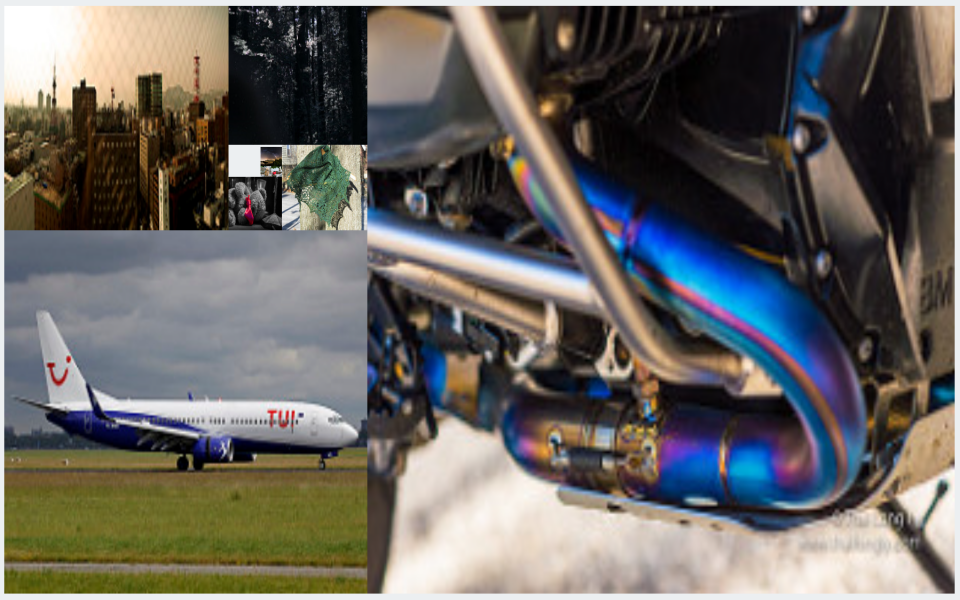
\includegraphics[width=\linewidth]{bluekittenflickr}
\caption[Image spiral `blue kitten'---Flickr]{Image spiral for query `blue kitten'---Flickr}
\label{fig:imgspiralflickr}
\end{figure}


\paragraph{Getty}
\begin{quotation}
  \begin{description}
    \item[keyword\_ids] Return only images tagged with specific keyword(s). Specify using a comma-separated list of keyword Ids. If keyword Ids and phrase are both specified, only those images matching the query phrase which also contain the requested keyword(s) are returned.
    \item[phrase] Search images using a search phrase.
  \end{description}
  \sourceatright{\autocite{GettyAPI}}
\end{quotation}

Getty uses the \py{phrase} parameter to set the query. It only creates one pataphysicalised query term from the original query and calls for ten results based on that. This decision was based on the quota restrictions\marginnote{§~\ref{s:quota}} defined by Getty. Their limit is based on calls per second rather than calls per day or month. This means we cannot run ten calls for each user query as we did with FLickr. The query ``blue kitten'' gets turned into the word ``racy'' which then calls the \ac{API} to retrieve ten results (see figure~\ref{fig:imgspiralgetty}\marginnote{§~\ref{fig:imgspiralgetty}}). The results mostly show racing cars from various angles although one oddball snuck in too: an office scene Getty has deemed to be `racy' (a guy in a suit checking out a lady's behind while she's leaning over a laptop).

\begin{figure}[!htbp]
\centering
  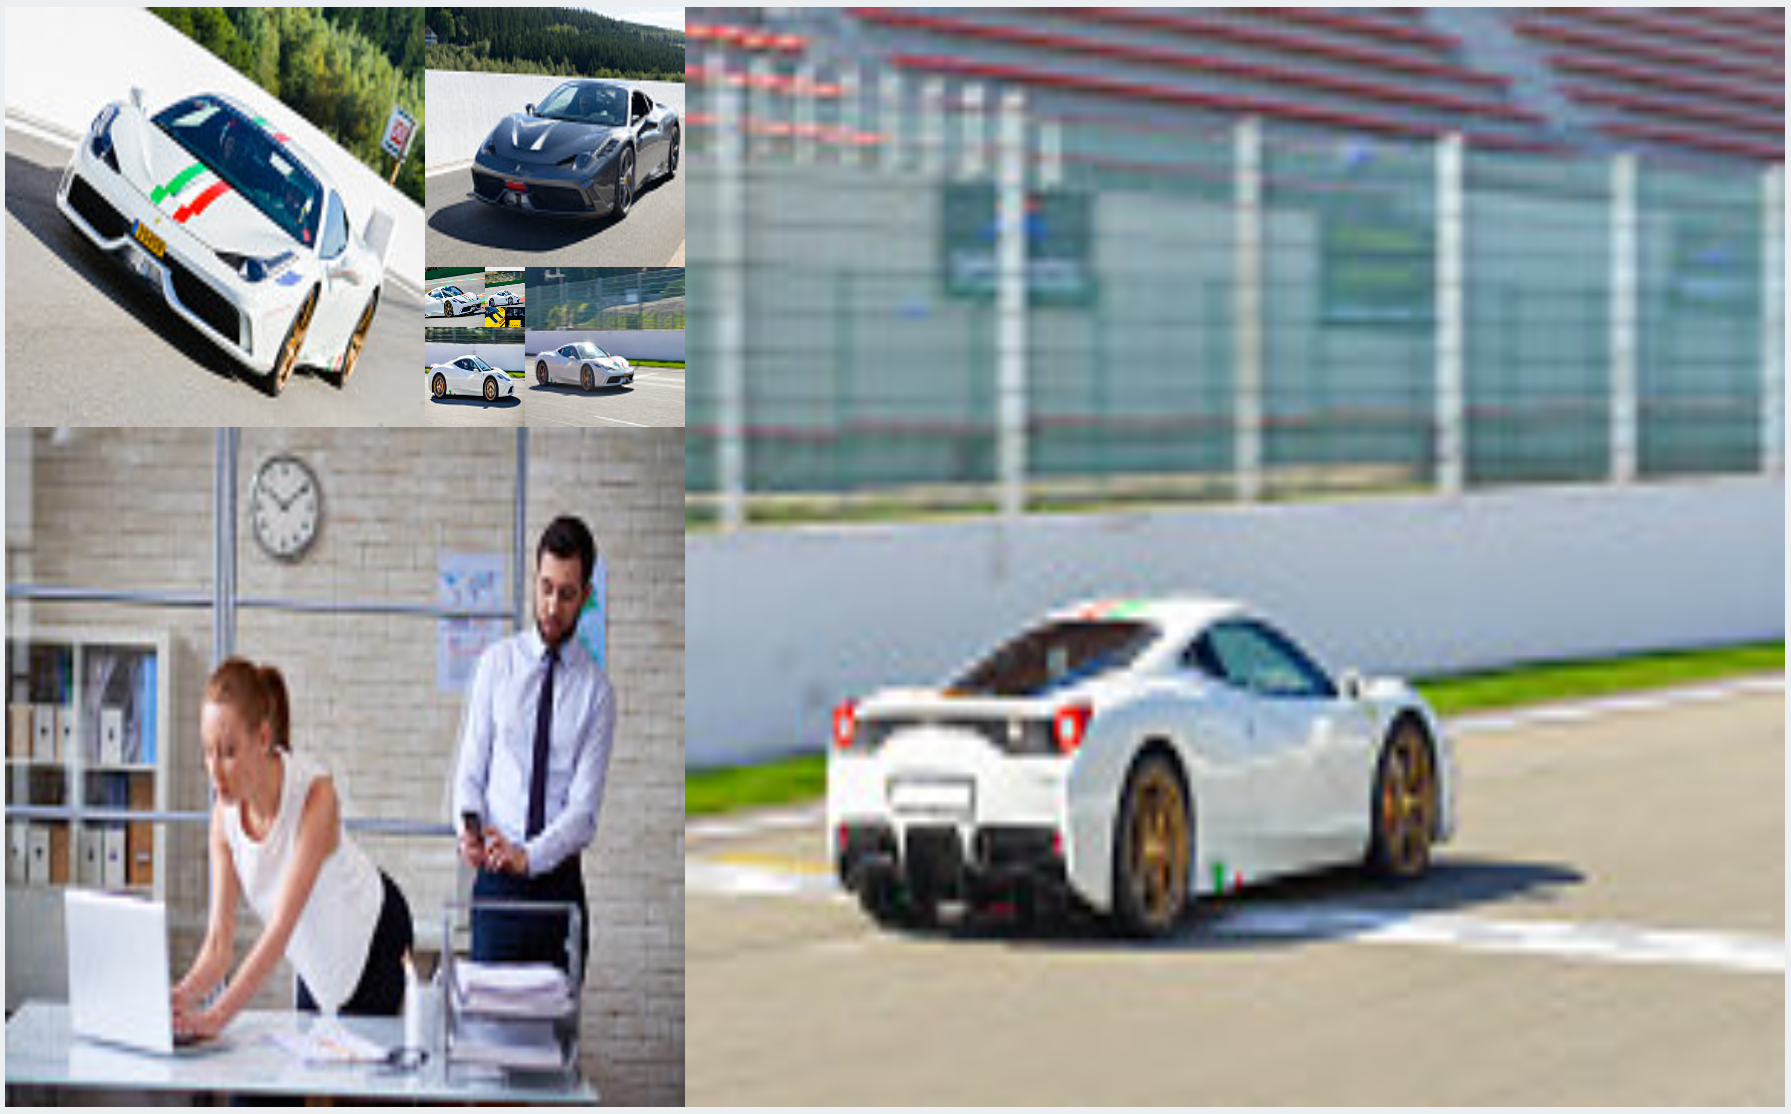
\includegraphics[width=\linewidth]{bluekittengetty}
\caption[Image spiral `blue kitten'---Getty]{Image spiral for query `blue kitten'---Getty}
\label{fig:imgspiralgetty}
\end{figure}

\paragraph{Bing}
\begin{quotation}
  \begin{description}
    \item[query] The user's search query string. The query string cannot be empty. The query string may contain Bing Advanced Operators\footnote{For example `AND', `OR', `imagesize:', `NOT', or `phrase'}. For example, to limit images to a specific domain, use the site: operator. To help improve relevance and the results, you should always include the user's query string in an insights query (see insightsToken). This parameter is supported only by the Image API; do not specify this parameter when calling the Trending Images API.
  \end{description}
  \sourceatright{\autocite{BingAPI}\footnote{Microsoft will discontinue this version of the current \ac{API} in December 2016. The new version is documented on \url{https://www.microsoft.com/cognitive-services/en-us/bing-image-search-api}.}}
\end{quotation}

For the Bing function uses the \py{query} parameter to set the query in the same way as Getty.

\paragraph{YouTube}
\begin{quotation}
  \begin{description}
    \item[q] The q parameter specifies the query term to search for. Your request can also use the Boolean NOT (-) and OR (|) operators to exclude videos or to find videos that are associated with one of several search terms. For example, to search for videos matching either ``boating'' or ``sailing'', set the q parameter value to boating|sailing. Similarly, to search for videos matching either ``boating'' or ``sailing'' but not ``fishing'', set the q parameter value to boating|sailing -fishing. Note that the pipe character must be URL-escaped when it is sent in your API request. The URL-escaped value for the pipe character is \%7C.
  \end{description}
  \sourceatright{\autocite{YouTubeAPI}}
\end{quotation}

Youtube works in a similar way as well. The \py{q} parameter is set to the pataphysicalised query term and one call retrieves ten results.

Something else to consider is perhaps that it is not entirely clear how the internal search for each \ac{API} works. This means that there's a possibility that they do their own query expansion\marginnote{§~\ref{s:qexpansion}} in the background to find more matches.


\subsubsection{Quota}
\label{s:quota}

Each \ac{API} has a different quota for their subscription packages. 

\begin{description}
  \item[Flickr] \num{3600} queries per hour are free \autocite{FlickrGuideAPI}.
  \item[Getty] \num{5} calls per second, unlimited calls per day \autocite{GettyOverviewAPI}.
  \item[Bing] \num{5000} transactions per month are free. A transaction is one request that returns one page of results \autocite{BingAzureAPI}.
  \item[YouTube] \num{50000000} units per day, \num{300000} units per \num{100} seconds per user, and \num{3000000} requests per \num{100} seconds are free. A call to the video search method counts as \num{100} units \autocite{YouTubeAPI}.
  \item[Microsoft Translator] \num{2000000} characters per month are free. Note the quota relates to single characters, not words \autocite{TranslatorAPI}.
\end{description}


\section{Formalisation}

A formal description of the \url{pata.physics.wtf} system in terms of an \ac{IR} model described in chapter~\ref{s:irmodels} is unsuitable.

Remember, an \ac{IR} model is a quadruple $[D,Q,F,R(q_i, d_j)]$ where:\\
\itab{$D$} \tab{is the set of documents,}\\
\itab{$Q$} \tab{is the set of queries,}\\
\itab{$F$} \tab{is the framework e.g.\ sets, Boolean relations, vectors}\\
\itab{}    \tab{~~~linear algebra\ldots}\\
\itab{$R(q_i, d_j)$}
            \tab{is the ranking function, where $q_i \in Q$ and $d_j \in D$,}\\
\itab{$t$} \tab{is the number of index terms in a document collection,}\\
\itab{$V$} \tab{is the set of all distinct index terms $\{k_1,\ldots, k_t\}$ in a document}\\
\itab{}     \tab~~~{collection (vocabulary).}

$D$ is the set of files we have in either the Faustroll or Shakespeare corpus. $Q$ is the given user query.



\section{Design}

It is interesting to note how different the search results are perceived when presented in a different style (e.g. list rather than poem). This could be studied using questionnaires and interviews or eye tracking tools to find out what users prefer or perceive as more creative for example (see chapter~\ref{ch:aspirations},~\ref{ch:aspirations}). 

\todo{feeling of ownership due to having to enter search term?}

Figures~\ref{fig:poemtree},~\ref{fig:listsourcetree}~and~\ref{fig:listalgotree} show the three different text result styles. The poetry\marginnote{\faicon{picture-o}~\ref{fig:poemtree}} is compact and invites users to read all 14 (or less) lines. The two list styles\marginnote{\faicon{picture-o}~\ref{fig:listsourcetree}~\&~\ref{fig:listalgotree}} are much longer and involve a lot of scrolling to navigate, which might deter users from actually reading many of the results.

\begin{figure}[!htbp]
\centering
  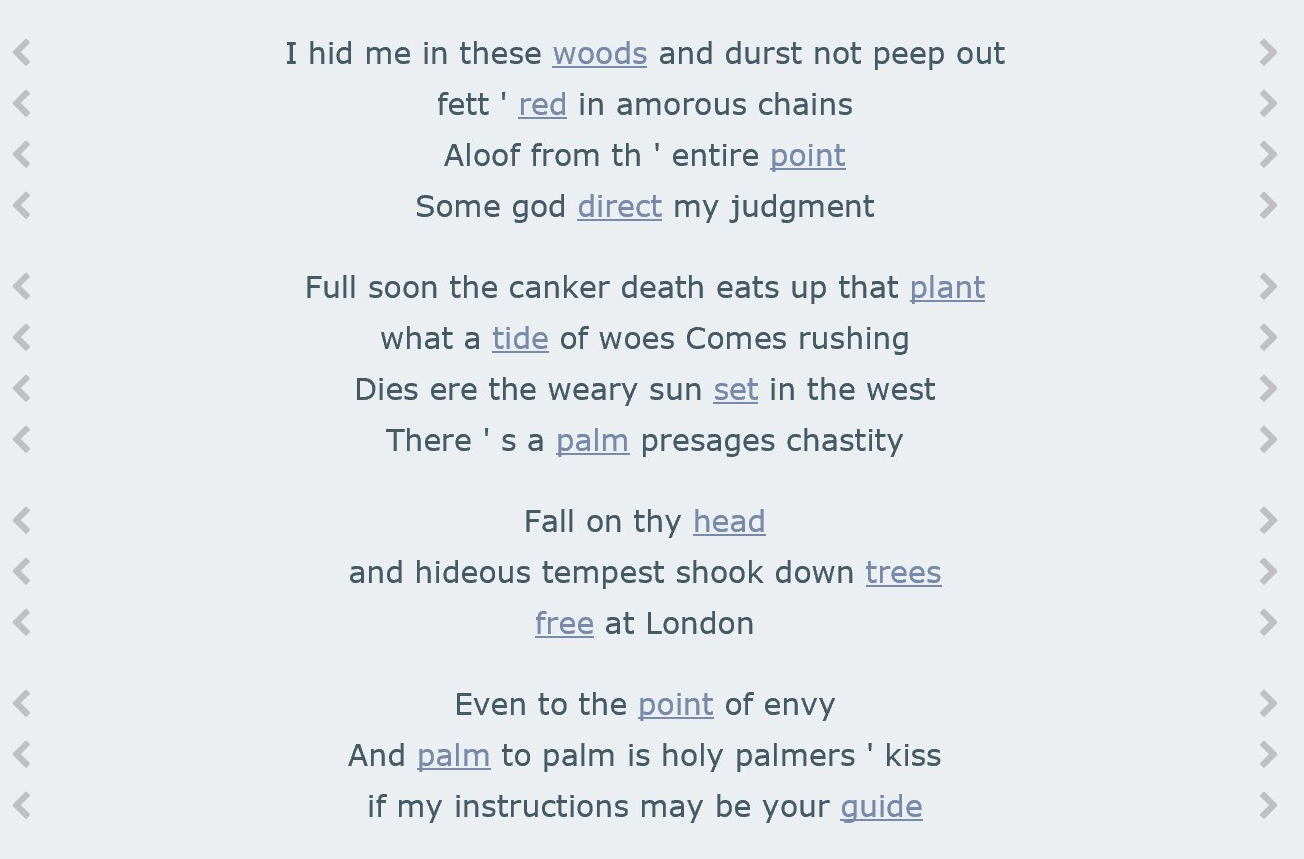
\includegraphics[width=\linewidth]{poemtree}
\caption[Results as poem]{Results in poem form for query `tree'---Shakespeare}
\label{fig:poemtree}
\end{figure}

\begin{figure}[!htbp]
\centering
  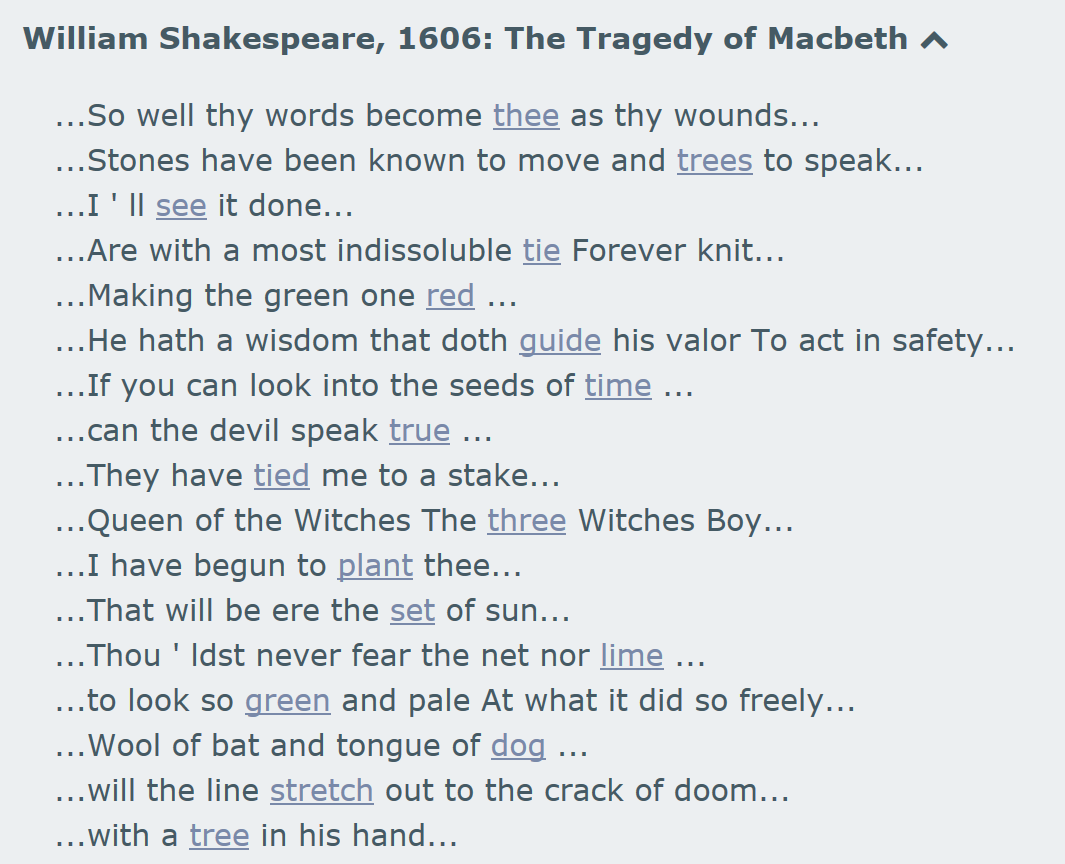
\includegraphics[width=\linewidth]{listsourcetree}
\caption[Results as list by sources]{Results as list by sources for query `tree'---Shakespeare}
\label{fig:listsourcetree}
\end{figure}

\begin{figure}[!htbp]
\centering
  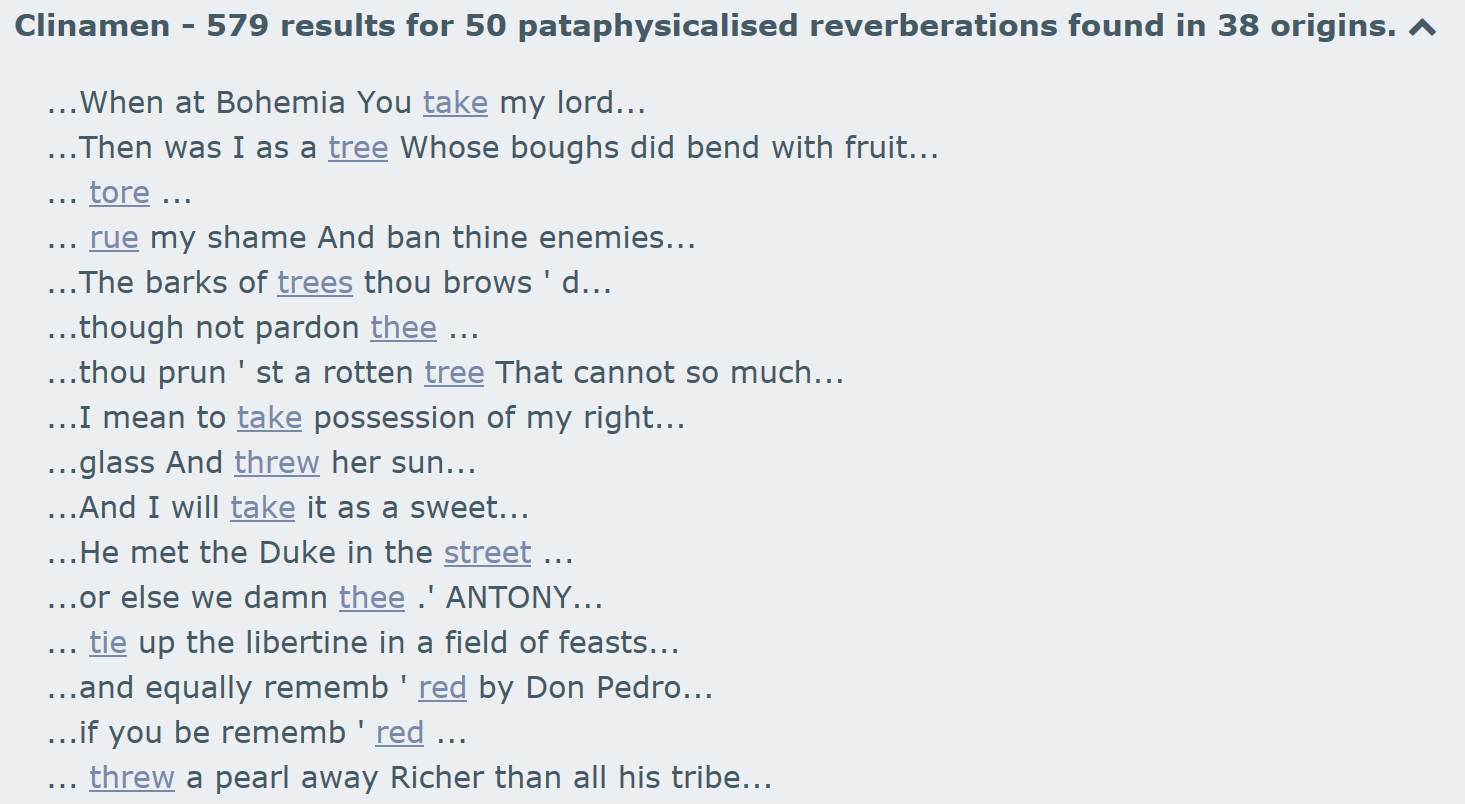
\includegraphics[width=\linewidth]{listalgotree}
\caption[Results as list by algorithm]{Results as list by algorithm for query `tree'---Shakespeare}
\label{fig:listalgotree}
\end{figure}


\section{Science Fiction}

A more theoretical question regarding the evolution of creative computing is related to developments in \ac{AI}. I have previously explored the similarities and differences 

HERE

Where does this project stand in the wider world and the progress of computing, \ac{AI} and creativity? \ac{AI} and robotics is alluring as a research topic because it is so prevelant in Science Fiction. Computer creativity rarely plays a centrol role though. We regularly read headlines that tell us that yet another kind of \ac{AI}-bot has won some game against a human player. Or we see videos of some innovative ground-breaking kind of new robot which claims to be near human-like (and yet cannot walk up stairs easily or hold a decent conversation). There are many examples of advances that are hailed as the next big thing which aren't all that great in the grand scheme of things. 

\subsection{AI}
This is also evident in games, for example \ac{VR} and \ac{AR}. The Oculus Rift and similar systems are advertised so much you might believe they are actually about to hit mainstream and every kid will own a \ac{VR} console and headset. Yet they are still way too expensive to be mainstream and motion sickness is also still an issue (and probably always will). These industries are so ``hip'' any publication is seen as the new cool thing without taking into account the history and work that has been done previously in perhaps slightly different disciplines. This is the case for example with a recent article on \ac{VR} sickness and how to compat it. This is a well known problem already---motion sickness already exists in normal games. Similar to epilepsy problems.

\todo{find links for motion sickness}
\todo{find links for epilepsy}
\todo{find links for oculus rift and pokenmon go etc}

\ac{AR} has very recently received a massive boom thanks to Pokenmon Go (released in Australia, New Zealand and the USA in July 2016). It has become a phenomenon since then.
\todo{find pokemon links}

What about IBM's Watson\footnote{See \url{http://www.ibm.com/watson/}}, Microsofts Twitter \ac{AI} chatbot Tay\footnote{See \url{https://web.archive.org/web/20160414074049/https://www.tay.ai/} for an archived version of the original website which is now offline. See also \url{https://twitter.com/tayandyou}, \url{https://www.theguardian.com/technology/2016/mar/24/tay-microsofts-ai-chatbot-gets-a-crash-course-in-racism-from-twitter}, and \url{https://www.theguardian.com/technology/2016/mar/30/microsoft-racist-sexist-chatbot-twitter-drugs}. Wikipedia also has a good article and sources on Tay: \url{https://en.wikipedia.org/wiki/Tay_(bot)}}, Google's AlphaGo\footnote{See \url{https://deepmind.com/alpha-go}} and Hanson Robotics Sophia robot\footnote{See \url{http://www.hansonrobotics.com/}}? How does this relate to my work? Practially of course they are all unrelated. On a deeper level though we can start asking interesting questions. 

https://www.engadget.com/2016/08/07/ibms-watson-ai-saved-a-woman-from-leukemia/
https://xkcd.com/1619/ XKCD WATSON

\begin{description}
  \item[IBM Watson] Watson is a question answering expert system. It famously won against human Jeopardy! champions in 2011.
  \item[Microsoft Tay] 
  \item[Google AlphaGo] AlphaGo is a system for playing the game Go. It won against a top human professional player in 2015.
  \item[Hansen Sophia]
\end{description}

I think these are interesting examples to study since they are supposedly on the forefront of \ac{AI} development. Life-like robots like Sophia still live in the `uncanny valley'. Her voice is creepy and unhuman, her intelligence or her capabilities if understanding conversations are clearly flawed (as shown by her viral remark about supporting genocide).\todo{check} Watson is clever and fast in finding answers for specific questions but he still had problems with humour (e.g. BLAHBLA\todo{find example}) but information lookup is arguably fairly easy and straightforward process within \ac{IR}---sure, it requires processing power and memory storage or access but it is based on simple matching of keywords, not any fancy heuristic algorithms. Microsofts twitter chatbot went viral and users `taught' it nasty swearwords \todo{check} quickly and Microsoft had to take the bot down. It has since apologised although any official documentation on it has disappeared \todo{check}. Google's AlphaGo has been hailed as a breakthrough in \ac{AI} but similar to Watson it is a very targeted and limited program. 

To me it seems the real breakthrough happens when (and if) the first robots appears which isn't as big as a house, can play Go, Chess and hide-and-seek, geniunely manages to get around he uncanny valley effect, has vast knowledge in his memory for instant information lookup, can hold a normal conversation without causing a war, etc, etc---you get the picture. General \ac{AI} is where it's at. Humans can do all the things we do. Children aren't born with only a single function. Imagine a world where humans only have one specialism and can;t do anything else. Mary is a Chess player but can't move her arms. Bob is a medical diagnosis expert but he can't hold a conversation. Movement, speech, memory---they are all vastly complex systems. And I haven't even touched creativity yet.

\todo{whats the point im making? how does this relate to my work?}
Perhpas this `uncanny valley' exists in creativity too. If a robot who looks vaguely human but not quite well enough, or he/she/it sounds almost human but not quite---perhaps if a robot can crack a joke like a human but not quite---perhaps this could be considered uncanny valley too? The philosphical zombies I mentioend in chapter~\ref{ch:interpretation}\marginnote{§~\ref{ch:interpretation}} live in this uncanny valley?

\todo{p and H creativity for computers?}


\subsection{Brains}

I'm not talking about the beer or the zombie food but rather research into the human brain (or animal brains) and attempts to model it on a computer. 

The motivation here is that once we understand how the brain works, perhaps we can understand how certain cognitive processes really work and this of course include creativity.

This is no easy task of course. Chris Chatham talks about ten ``important Differences Between Brains and Computers''\footnote{\url{http://scienceblogs.com/developingintelligence/2007/03/27/why-the-brain-is-not-like-a-co/}} which give a good overview of some of the dificulties of trying to model a brain as is. We can't just do a 1-1 copy.

\begin{quotation}
  \begin{enumerate}
    \item Brains are analogue; computers are digital
    \item The brain uses content-addressable memory
    \item The brain is a massively parallel machine computers are modular and serial
    \item Processing speed is not fixed in the brain; there is no system clock
    \item Short-term memory is not like RAM
    \item No hardware/software distinction can be made with respect to the brain or mind
    \item Synapses are far more complex than electrical logic gates
    \item Unlike computers, processing and memory are performed by the same components in the brain
    \item The brain is a self-organising system
    \item Brains have bodies
    \item	The brain is much, much bigger than any [current] computer
  \end{enumerate}
\sourceatright{Chris Chatham}
\end{quotation}

To bring this into perspective Ray Kurzweil claims the brain is capable of $10^{16}$ operations per second \citeyear[p.194]{Kurzweil2013}. Japan's K-computer (the worlds largest super computer as of 2016) currently has that power---10 petaflops. The ``Blue Brain Project'' is aiming to model $10^17$ bytes of memory and $10^{18}$ flops by 2023 \autocite[p.125]{Kurzweil2013}.
\todo{find k-computer reference}

There are currently some major research projects going on. One of them is the ``Human Brain Project'' \autocite{Walker2012}.

\begin{draft}
quotes:

Our brain consumes about 30W, the same as an electric light bulb, thousands of times less than a small supercomputer. \autocite[p.17]{Walker2012}

For environmental and business reasons, vendors have set themselves the goal of containing energy consumption to a maximum of 20 megawatts  \autocite[p.41]{Walker2012}

the 1 PFlop machine at the Jülich Supercomputing Centre could simulate up to 100 million neurons – roughly the number found in the mouse brain. \autocite[p.41]{Walker2012}

Cellular-level simulation of the 100 billion neurons of the human brain will require compute power at the exascale (1018 flops). \autocite[p.41-42]{Walker2012}

2017 petascale 50petabytes memory + 50 petaflops + <=4MW power

2021 exascale 200petabyte memory + 1exaflop

A second, equally important goal will be to prepare the procurement of the HBP Pre-exascale-supercomputer. By 2017/18, Jülich plans to procure a Big Data-centred system with at least 50 PBytes of hierarchical storage-class memory, a peak capability of at least 50 PFlop/s and a power consumption <= 4 MW. The memory and computational speed of the machine will be sufficient to simulate a realistic mouse brain and to develop first-draft models of the human brain. (The rest of the hardware roadmap targets an exascale machine in 2021/2022 with a capability of 1 EFlop/s and a hierarchical storage-class memory of 200 PB).\footnote{https://www.humanbrainproject.eu/high-performance-computing-platform}

\end{draft}

Why Minds Are Not Like Computers \autocite{Schulman2009}
Software – Hardware == Mind – Brain ??? analogy

"The power of the computer derives not from its ability to perform complex operations, but from its ability to perform many simple operations very quickly."

Layers of abstraction in computers:\\
1.	user interface\\
2.	high level programming language\\
3.	machine language\\
4.	proessor microarchitecture\\
5.	Boolean logic gates\\
6.	transistors\\

layers of abstraction in brain:\\
1.	personality?\\
2.	Thinking?\\
3.	Chemical /electrical signals/activity?\\
4.	Divided Brain regions/structure\\
5.	Neurons\\
6.	Dendrites (input) and axons (output)?\\


Computers are faster and better than humans in many tasks already.

\begin{quote}
"The weaknesses of the computational approach include its assumption that cognition can be reduced to mathematics and the difficulty of including noncognitive factors in creativity." \autocite[p.457]{Mayer1999}
\end{quote}

\todo{find references}
\todo{neural networks and other models based on the brain}

Perhaps we need to have that complete picture of how the brainw orks in order to understand human creativity. I would argue computer creativity is part of general \ac{AI}, and for general \ac{AI} we need massive amounts of general knoweldge.
\todo{common sense research}
\todo{again talk about how this is relevant for my project}
\paragraph{Expert Systems vs General AI}
Is computer creativity an expert system or does it fall into general \ac{AI}? 

\paragraph{Machines self-assessing}
Perhaps there is an argument that if humans are the only entities who can judge whether another human is being creative, then machines should be assessing themselves. This is a paradoxical concepts though. Since machines are products made my humans, they can never be autonomous in that sense. If machines had evolved like other animals besides us this argument might hold but obviously that is not the case.



\section{Meta}

\subsection{Management}
\todo{add file for appendix with full git history}

On a different note, the project was completed over X years which includes an interruption and later on only a part time commitement.

I kept the project in a ``git repository''. Git is a version ontrol system that allows users to roll-back on changes and I further pushed my work to GitHub to make sure hardware failure or human error (i.e. lost or stolen property) would not affect my work. 

To understand git you need to know what commits are. They are the thing where I save my current state of the project and give it a description.

Below you can see a shortened version of the timeline of my commits between 20XX and the time of submission of this thesis. A full version can be found in appendix XYZ. You can see from this the time between programming work I did on \url{pata.physics.wtf} and its predecessors.

\todo{add calendar screenshot of github contributions}
\todo{links to git and github}

\begin{verbatim}
  *   10f61f9  Sun 08 May 2016	 (HEAD -> api, origin/api) Merge remote-tracking branch 'refs/remotes/origin/master' into api
  |\  
  * | 71437f6  Tue 18 Aug 2015	 Flickr and Bing work, radio buttons work
  * | 6c552aa  Wed 12 Aug 2015	 Fixed image problem but not video.
  | | * 1cbb63d  Tue 11 Aug 2015	 (origin/thesis) Update textsurfer.py
  | |/  
  |/|   
  * | 0ebff0d  Tue 11 Aug 2015	 Analytics enabled again
  * | 703f977  Tue 11 Aug 2015	 Problems solved.
  * | 74a1fae  Tue 11 Aug 2015	 About to change l\_dict to dict of dict
  * | 0935b23  Mon 10 Aug 2015	 BUG FUCKER
  * | 4f7d91e  Mon 10 Aug 2015	 Turn debug off
  * | 58f0c2b  Mon 10 Aug 2015	 Button styling done
  * | 59add58  Mon 10 Aug 2015	 Email problem solved
  * |   f1b2d40  Sun 09 Aug 2015	 Merge branch 'Deploy' into thesis
  |\ \  
  | * | 435cb2d  Sun 09 Aug 2015	 Deployment works, added analytics
  | * | 8a63dc7  Sat 08 Aug 2015	 gunicorn runs locally fine.
  | * | 2861407  Sat 08 Aug 2015	 Revert 5f2c957..4026965
  | * | 4026965  Sat 08 Aug 2015	 Tests
  * | |   8f2eeab  Sat 08 Aug 2015	 Merge branch 'w3' into thesis
  |\ \ \  
  | |/ /  
  | * | 5f2c957  Sat 08 Aug 2015	 Stuff
  | * | 873153c  Fri 07 Aug 2015	 Tiny cleanup
  | * | 05d5760  Thu 06 Aug 2015	 Random Poems and Emailing works
  | * | 657126c  Wed 05 Aug 2015	 Random poems work - without links though
  | * | 3d31ea9  Wed 05 Aug 2015	 Randomise still only works once, count ok
  | * | 5f1d45b  Wed 05 Aug 2015	 Randomise poem works ONCE
  | * | c583341  Wed 05 Aug 2015	 Poem subtabs, email poems done
  | * | f1b3878  Wed 05 Aug 2015	 Hiding divs
  | * | a6939c4  Tue 04 Aug 2015	 huh?
  | * | e6b411d  Tue 04 Aug 2015	 Poem emails WORK Fuck YEAH!
  | * | 4b6b170  Tue 04 Aug 2015	 Test email
  | * | 24e356c  Tue 04 Aug 2015	 Better load icon
  | * | e6ae736  Tue 04 Aug 2015	 loading icon version 1
  | * | 51b43e2  Tue 04 Aug 2015	 Added 4th pictures
  | * | f2d8a83  Mon 03 Aug 2015	 Minor fixes
  * | |   1ddb03d  Mon 03 Aug 2015	 Merge branch 'w3' into thesis
  |\ \ \  
  | |/ /  
  | * | ca4eab3  Mon 03 Aug 2015	 Pretty good state.
  | * | 9370334  Mon 03 Aug 2015	 working on list display of images
  | * | e1f1ead  Mon 03 Aug 2015	 Stylesheets sorted and cleaned files
  * | |   9732d5b  Mon 03 Aug 2015	 Merge branch 'w3' into thesis
  |\ \ \  
  | |/ /  
\end{verbatim}

\spirals

I also kept the thesis under git version control. Since the thesis was written in \LaTeX you could almost say I `programmed' it. Below is an outline of the commit history for this thesis.

\begin{verbatim}
* 3f06260	 Edited readme again
* c721b33	 Edited readme
* ffbdb4b	 Edited readme
* 8870b3d	 Added gitignore file
* ba1a9c2	 Second commit
* 244c4b3	 First commit
\end{verbatim}


\subsection{Thesis}

\subsubsection{Part Spirals}

Each new thesis part contains a word spiral based on a poem generated by \url{pata.physics.wtf} using the a part of the title as keyword. They represent the pataphysical (Archimedean) spiral.

\begin{enumerate}
  \item Preface --- \emph{pre}
  \item Hello World --- \emph{hello}
  \item Tools of the Trade --- \emph{trade}
  \item The Core: Techno-Logic --- \emph{core}
  \item The Core: Techno-Practice --- \emph{practice}
  \item Meta-Logicalysis --- \emph{meta}
  \item Happily Ever After --- \emph{after}
  \item Postface --- \emph{post}
\end{enumerate}

\subsubsection{Chapter Poetry}

Each chapter opens with a poem generated by \url{pata.physics.wtf} using a part of the chapter title as keyword.

\begin{enumerate}
  \item Introduction --- \emph{intro}
  \item Inspirations --- \emph{inspiration}
  \item Methodology --- \emph{method}
  \item Pataphysics --- \emph{pata}
  \item Creativity --- \emph{creativity}
  \item Technology --- \emph{technology}
  \item Evaluation --- \emph{evaluation}
  \item Foundations --- \emph{foundation}
  \item Interpretation --- \emph{interpretation}
  \item Implementation --- \emph{implementation}
  \item Applications --- \emph{application}
  \item Patanalysis --- \emph{patanalysis}
  \item Aspirations --- \emph{aspirations}
  \item Observations --- \emph{observations}
\end{enumerate}

\todo{say more, check keywords, potentially generate new poems}





\section*{creative analysis}
\begin{draft}
  literary deconstruction and recombining to make new creative output? \\
  perception of results (poetry, source, algorithm) \\
  discuss applications from before (stimulates creative detour away from the obvious) \\

  How does this relate to Oulipo and Pataphysics? 

  Perhaps this is where I should talk a bit about the perception of results in their different output formats/styles. The poetry is automatically read with more gravity. Sorting by sources is a game of exploration or algorithms which becomes a game of finding the similarities within the result sets. They are different ways to view the same things and yet have a drastic influence of how the results are perceived. This also applies to the image and video search. Presenting results in spiral form is weird. Its hard to see where one image ends and another starts, they just kind of blur into each other. When listed as a list they immediately become more boring.

  talk abit about what the original plan was for some of the big changed elements in the website, e.g. the image search running 10 times on different keywords rather than running once with 10 results for the same keyword.
\end{draft}


DELETE EVERYTHING FROM BELOW HERE:


\begin{draft}
DELETE THIS

In this section we consider the possible uses and applications for the proposed creative search tool.

Our target audience is not quite as broad as that of a general search engine like Google. Instead, we aim to specifically cater for users who can appreciate creativity or users in need of creative inspiration. Users should generally be educated about the purpose of the search tool so that are not discouraged by what might appear to be nonsensical results. Users could include artists, writers or poets but equally anybody who is looking for out-of-the-box inspirations or simply a refreshingly different search engine to the standard.

The way we display and label results produced by the tool can influence how the user perceives them. The current prototype for example separates the results into its three components but we could have equally just mixed them all together. The less transparent the processes in the background (e.g.\ which algorithm was used, how does the result relate to the query precisely, etc.) are for the user, the more difficult it might be to appreciate the search.

There are many ways a pataphysical search tool could be used across disciplines.

In literature, for example, it could be used to write or generate poetry, either practically or as a simple aid for inspiration. We are not limited to poetry either; novels, librettos or plays could benefit from such pataphysicalised inspirations. One can imagine tools using this technology that let you explore books in a different ordering of sentences (a sort of pataphysical journey of paragraph hopping), tools that re-write poems or mix and match them together. Even our simple prototype shows potential in this area and could be even more powerful if we extended it to include more base texts, for example the whole set of books contained in Faustroll’s library ([20] and also [12]). A richer body of texts (by different authors) would produce a larger index which would possibly find many more matches through WordNet and end in a more varied list of results.

From a computer science perspective it could be used as one of the many algorithms used by traditional search engines for purposes like query feedback or expansion (e.g. “did you mean … “or “you might also be interested in … “). Depending on how creative we want the search engine to be, the higher we would rank the importance of this particular algorithm. One of the concepts related to the search tool, namely patadata, could have an impact on the development of the Semantic Web. Just as the Semantic Web is about organizing information semantically through objective metadata, patadata could be used to organize information pataphysically in a subjective way.

The prototype tool is already being used in the creation of an online opera, provisionally entitled from [place] to [place], created in collaboration with The Opera Group, an award-winning, nationally and internationally renowned opera company, specialising in commissioning and producing new operas. In particular, it is being used to create the libretto for one of the virtual islands whose navigation provides the central storyline for the opera. The opera will premiere in 2013, and will continue to develop thereafter, deploying new versions of the tool as they appear.
\end{draft}






\stopcontents[chapters]
